% main7.tex -- H-main.  Section 7: from eps > 0 to exact capture.
%======================================================================
\section{From $\varepsilon>0$ to exact capture}\label{sec:exact}
%======================================================================

Theorem~\ref{thm:main} gives, for every vision radius $\varepsilon$, a path that sees every direction by the same time
$T_0d$. All these paths are $1$-Lipschitz on the common interval $[0,T_0d]$, so a subsequence converges uniformly as
$\varepsilon\to0$ (Figure~\ref{fig:limit}). If the limit path missed some direction, that candidate would stay a positive
distance away from it; by continuity it would also stay away from the nearby paths with tiny $\varepsilon$, which is
impossible. This is why the uniformity of the time bound in $\varepsilon$ is the crux of the whole paper: if the search
time grew as $\varepsilon\to0$, there would be no common interval and no limit.

\begin{figure}[!htbp]
\centering
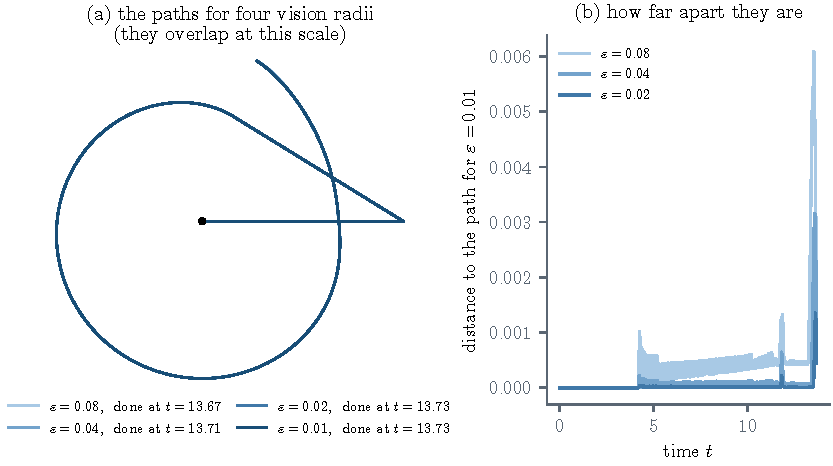
\includegraphics[width=0.95\linewidth]{figs/fig_limit.pdf}
\caption{The paths of the proof for four vision radii ($v=0.1$, simulated). (a) They are indistinguishable at this
scale, and all finish at about the same time. (b) Their distance from the path for $\varepsilon=0.01$; it shrinks
with $\varepsilon$, except for spikes near the end of the walk, which come from different final legs. The exact catch of Corollary~\ref{cor:exact} comes from a limit of such paths.}
\label{fig:limit}
\end{figure}

\begin{lemma}[Compactness]\label{lem:compact}
Let $d>0$, let $D_1\subset D_2\subset\cdots$ be finite sets of directions whose union is dense in $[0,2\pi)$, and let
$\varepsilon_N\to0$. Suppose that for each $N$ a $1$-Lipschitz path $H_N$ with $H_N(0)=0$ comes within $\varepsilon_N$ of
every candidate $S_\alpha$, $\alpha\in D_N$ \textup(the candidates for the path $H_N$\textup), by a time $\bar T$
independent of $N$. Then there is a $1$-Lipschitz path $H$ with $H(0)=0$ that catches every direction by time $\bar T$.
\end{lemma}

\begin{proof}
By the Arzel\`a--Ascoli theorem a subsequence, still written $H_N$, converges uniformly on $[0,\bar T]$ to a
$1$-Lipschitz path $H$ with $H(0)=0$. For a $1$-Lipschitz path $G$ write $\rho^G_\alpha:=|S_\alpha-G|$, where $S_\alpha$ is
the candidate $\alpha$ for the path $G$; it is defined until the catch, and $|(\rho^G_\alpha)'|\le1+v$. We use the
elementary inequality $|y/|y|-z/|z||\le2|y-z|/\max(|y|,|z|)$.

\emph{Claim.} Let $G,G_k$ be $1$-Lipschitz paths on $[0,\bar T]$ with $\|G_k-G\|_\infty\to0$, and suppose
$\rho^G_\alpha\ge c>0$ on $[0,\tau]$, $\tau\le\bar T$. Put $\tau':=\min(\tau+c/(2(1+v)),\bar T)$. Then there are a
neighbourhood $\mathcal U$ of $\alpha$ and a $k_0$ such that for $\alpha'\in\mathcal U$ and $k\ge k_0$ the candidate
$\alpha'$ for $G_k$ is defined on $[0,\tau']$ and $\rho^{G_k}_{\alpha'}\ge c/4$ there.

Indeed, since $|(\rho^G_\alpha)'|\le1+v$, the candidate $S:=S_\alpha$ for $G$ is defined on $[0,\tau']$ with
$\rho^G_\alpha\ge c/2$ there. Let $\tilde S:=S_{\alpha'}$ be the candidate for $G_k$. As long as
$|S-G|,|\tilde S-G_k|\ge c/4$, the inequality above gives
$|\tilde S-S|(t)\le|\tilde S-S|(0)+(8v/c)\int_0^t\bigl(|\tilde S-S|+\|G_k-G\|_\infty\bigr)$, so by Gr\"onwall's
inequality $|\tilde S-S|\le b_k:=\bigl(|e^{i\alpha'}-e^{i\alpha}|d+(8v/c)\bar T\|G_k-G\|_\infty\bigr)e^{8v\bar T/c}$.
Choose $\mathcal U$ and $k_0$ with $b_k+\|G_k-G\|_\infty<c/4$. Let $I$ be the set of $s\in[0,\tau']$ such that $\tilde S$
is defined on $[0,s]$ with $|\tilde S-G_k|\ge c/4$ there. Then $0\in I$ (as $|\tilde S(0)-G_k(0)|=d\ge c$), $I$ is
closed (as $|\tilde S'|=v$, $\tilde S$ extends continuously to $\sup I$, where $|\tilde S-G_k|\ge c/4>0$ still holds,
so it is defined there), and for $s\in I$ the bound gives $|\tilde S-G_k|\ge|S-G|-b_k-\|G_k-G\|_\infty>c/4$ on $[0,s]$, so $I$ also
contains a neighbourhood of $s$ in $[0,\tau']$. Hence $I=[0,\tau']$, proving the claim.

Now fix $\alpha\in D_M$. For $N\ge M$ we have $\alpha\in D_N$; let $t_N\le\bar T$ be the first time with
$\rho^{H_N}_\alpha(t_N)\le\varepsilon_N$, and pass to a subsequence with $t_N\to t^*\le\bar T$. If $H$ did not catch
$\alpha$ by time $t^*$, then $\rho^H_\alpha$ would be defined and positive on $[0,t^*]$, hence $\ge c>0$ there, and
the claim (with $G=H$, $G_k=H_N$, $\alpha'=\alpha$, $\tau=t^*$) would give $\rho^{H_N}_\alpha\ge c/4$ on
$[0,\min(t^*+c/(2(1+v)),\bar T)]$, an interval containing $t_N$ for large $N$; this contradicts $\varepsilon_N\to0$.
So $H$ catches every direction of $\bigcup_ND_N$ by time $\bar T$. Finally, the claim with $G_k=G=H$ and $\tau=\bar T$
shows that the set of directions \emph{not} caught by $H$ on $[0,\bar T]$ is open. It is disjoint from the dense set
$\bigcup_ND_N$, hence empty.
\end{proof}

\begin{proof}[Proof of Corollary~\ref{cor:exact}]
By scaling we may take $d=1$. Fix $v\in(0,v_0]$ and apply Lemma~\ref{lem:compact} with $\bar T:=T_0$,
$D_N:=\{2\pi i/2^N:0\le i<2^N\}$, $\varepsilon_N:=2^{-N}\varepsilon_*$, and $H_N$ the path of Theorem~\ref{thm:main}
for $(v,\varepsilon_N,1)$. Theorem~\ref{thm:main} says exactly that $H_N$ comes within $\varepsilon_N$ of every candidate
by time $T_0$, so the lemma gives a single path that catches every direction by time $T_0$.
\end{proof}

\textbf{What the proof does not give.} The argument is qualitative in $v$: it shows that \emph{some} $v_0>0$ works, and
the companion paper \cite{short} shows that $v_0=5.8\cdot10^{-3}$ does, with explicit constants checked by computer. The
simulations suggest that Design~T followed by the walk succeeds for much larger $v$, but we have no estimate of how
large $v$ may be for the method itself. The limit path of Corollary~\ref{cor:exact} is not explicit.
